\documentclass[a4paper, 11pt]{article}
\usepackage[utf8]{inputenc}
\usepackage[left=2cm, right=2cm, top=2cm]{geometry}
\usepackage{graphicx}
\usepackage{listings}
\usepackage{amsmath}
\usepackage{ulem}
\usepackage{xcolor}
\usepackage[backref]{hyperref}
\usepackage{caption}
\usepackage{subcaption}
\usepackage{float}
\usepackage{amssymb}
\usepackage{algorithm}
\usepackage{algpseudocode}

\hypersetup{
  colorlinks,
%   allcolors=blue,
%   urlcolor=blue,
}

\definecolor{codegreen}{rgb}{0,0.6,0}
\definecolor{codegray}{rgb}{0.5,0.5,0.5}
\definecolor{codepurple}{rgb}{0.58,0,0.752}
\definecolor{backcolour}{rgb}{0.95,0.95,0.92}
\lstdefinestyle{mystyle}{
    backgroundcolor=\color{backcolour},   
    commentstyle=\color{codegreen},
    keywordstyle=\color{magenta},
    numberstyle=\tiny\color{codegray},
    stringstyle=\color{codepurple},
    basicstyle=\ttfamily\footnotesize,
    breakatwhitespace=false,         
    breaklines=true,                 
    captionpos=b,                    
    keepspaces=true,                 
    numbers=left,                    
    numbersep=5pt,                  
    showspaces=false,                
    showstringspaces=false,
    showtabs=false,                  
    tabsize=2
}

\renewcommand*\contentsname{Table of Contents}

\begin{document}

\let\endtitlepage\relax
\begin{titlepage}
   \begin{center}

    	% \includegraphics[width=3cm, height=3cm]{habib-Logo.jpeg}

       \vspace*{0.5cm}

        \LARGE\textbf{Assignment 3 : Reinforcement Learning and Self-organizing Maps}\\
        \vspace{0.2cm}
       \large\textbf{Computational Intelligence}\\
       \vspace{0.2cm}
       \textbf{Spring 2021}\\
       \vspace{0.2cm}
            
       \textbf{Munawwar Anwar Adam \\Khubaib Naeem Kasbati}
   \end{center}
\end{titlepage}
\noindent\makebox[\linewidth]{\rule{\textwidth}{0.4pt}}
\tableofcontents
\noindent\makebox[\linewidth]{\rule{\textwidth}{0.4pt}}
\newpage
\section{Question 1: Value Iteration}
\subsection{Problem Description and Solution}
Our goal is to create a value iteration agent that takes the best possible path to a reward and stays away from obstacles, while minimizing movement. \\
In order to minimize movement, we set values which are neither reward nor obstacles immediate payoff as -1 to discourage additional movement. Reward was given the value of $+100$ while Obstacle was given the value $-100$. Using the value iteration algorithm, optimum values were found.
\subsection{Results}
We tested our output on multiple grids, in order to ensure optimal results. \\ 
In Grid \ref{fig:grid1}, we can see that the obstacles are avoided and the shortest path is being taken. \\
In Grid \ref{fig:grid2}, we set 4 rewards, one for each corner. Over here, we can see that the agent's decision depends on which quadrant it is in and it approaches the reward that is closest to it, showing it has learned to minimize movement. \\
In Grid \ref{fig:grid3}, we can see a similar setup, however, movement near the top left is restricted due to obstacles. It is seen that our Value iteration agent has learned that there is an obstacle and decides to approach another reward. \\
In Grid \ref{fig:grid4}, we have placed several obstacles and one goal near the obstacles. Our value iteration agent has learned this and is optimally going towards the goal. We can see that on the right side of the obstacle cluster, the agent sticks near the obstacles in order to prevent unnecessary movement showing optimal behaviour.
\begin{figure*}[h!]
    \centering
    \begin{subfigure}[t]{0.5\textwidth}
        \centering
        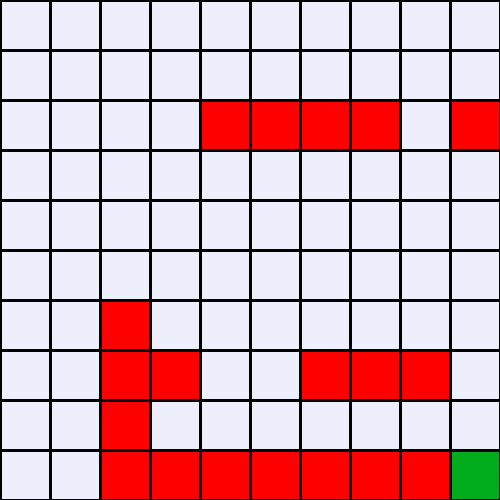
\includegraphics[width=0.75\textwidth]{Images_Q1/grid1_default.png}
        \caption{Grid without Policy}
    \end{subfigure}%
    ~ 
    \begin{subfigure}[t]{0.5\textwidth}
        \centering
        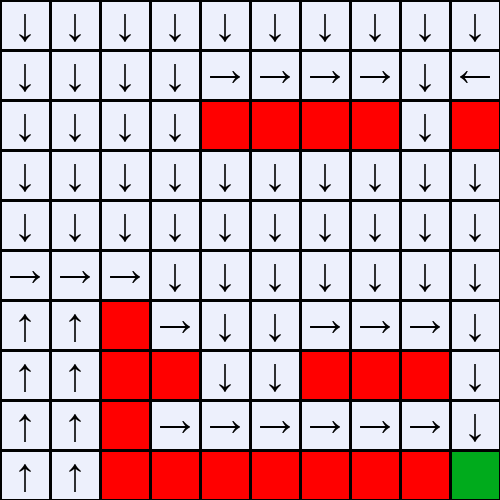
\includegraphics[width=0.75\textwidth]{Images_Q1/grid1.png}
        \caption{Grid with Policy}
    \end{subfigure}
    \caption{Grid 1}
    \label{fig:grid1}
\end{figure*}
\newpage
\begin{figure*}[h!]
    \centering
    \begin{subfigure}[t]{0.5\textwidth}
        \centering
        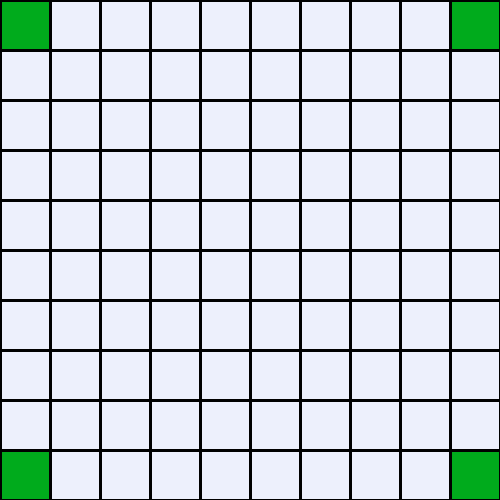
\includegraphics[width=0.75\textwidth]{Images_Q1/grid2_default.png}
        \caption{Grid without Policy}
    \end{subfigure}%
    ~ 
    \begin{subfigure}[t]{0.5\textwidth}
        \centering
        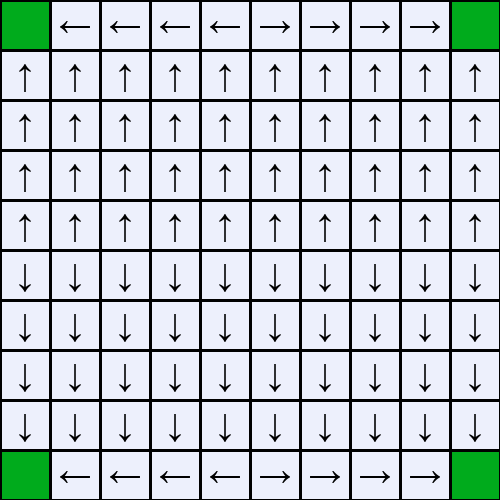
\includegraphics[width=0.75\textwidth]{Images_Q1/grid2.png}
        \caption{Grid with Policy}
    \end{subfigure}
    \caption{Grid 2}
    \label{fig:grid2}
\end{figure*}
\begin{figure*}[h!]
    \centering
    \begin{subfigure}[t]{0.5\textwidth}
        \centering
        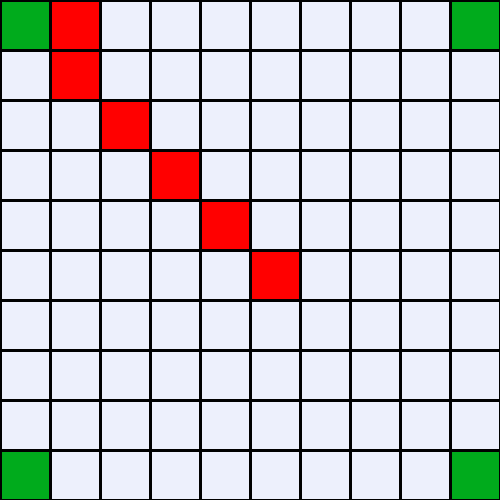
\includegraphics[width=0.75\textwidth]{Images_Q1/grid3_default.png}
        \caption{Grid without Policy}
    \end{subfigure}%
    ~ 
    \begin{subfigure}[t]{0.5\textwidth}
        \centering
        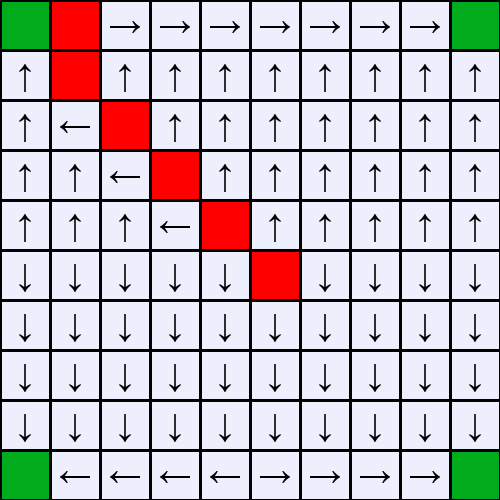
\includegraphics[width=0.75\textwidth]{Images_Q1/grid3.png}
        \caption{Grid with Policy}
    \end{subfigure}
    \caption{Grid 3}
    \label{fig:grid3}
\end{figure*}
\begin{figure*}[h!]
    \centering
    \begin{subfigure}[t]{0.5\textwidth}
        \centering
        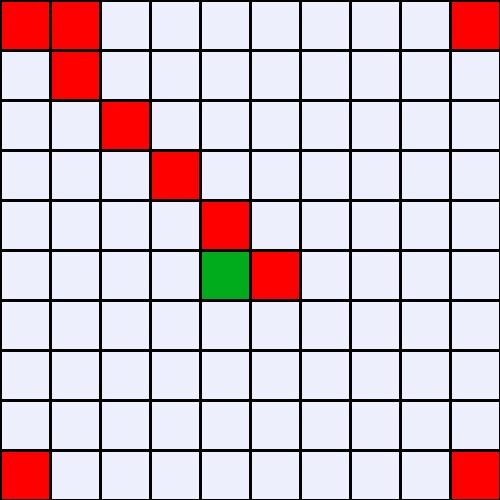
\includegraphics[width=0.75\textwidth]{Images_Q1/grid4_default.png}
        \caption{Grid without Policy}
    \end{subfigure}%
    ~ 
    \begin{subfigure}[t]{0.5\textwidth}
        \centering
        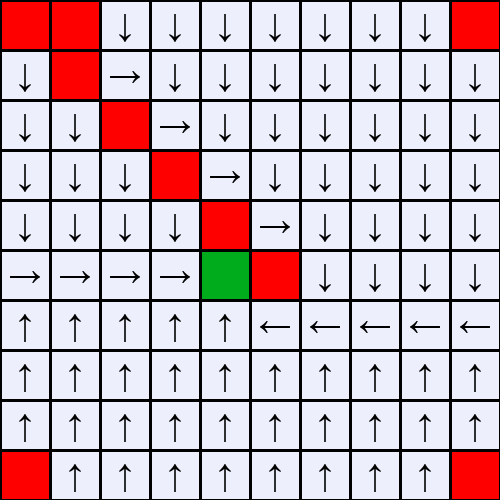
\includegraphics[width=0.75\textwidth]{Images_Q1/grid4.png}
        \caption{Grid with Policy}
    \end{subfigure}
    \caption{Grid 4}
    \label{fig:grid4}
\end{figure*}
\newpage
\section{Question 2: Self Organising Maps}
\subsection{Introduction}
Self-Organizing Map (SOM) is an unsupervised neural network model. It is for clustering, dimension reduction, and feature detection. SOM is used for data visualization by projecting higher dimensional data into lower dimensional space leveraging topological similarity properties. While learning the model, SOM utilizes competitive learning techniques. 
\subsection{Problem Description and Solution}
Our goal is to visualize the dataset``Total World Population by Gender from 1950 to 2100''. The features that we will be considering to cluster this data are \textbf{Total Population},\textbf{Population Density},\textbf{Population Female} and \textbf{Population Male}.
\newline
The Kohenon network consists of $10 \times 10 $ nodes where each node is connected to the input layer which is representing a four dimension input vector. The four dimensions of the input correspond to the four features that we are considering. The values of the rest of the parameters is as follows :
\begin{itemize}
    \item Number of Iterations : 20,000
    \item Initial Learning Rate : 0.01
    \item Initial Radius : 5
\end{itemize}
The exponential decay function for finding the neighborhood size is as follows:
$$ \sigma(t) = \sigma_0 \times e^{-(\frac{t}{ \lambda})}$$
where $\sigma_0$ is the initial radius, $t$ is the time step and $\lambda$ is the time constant. 
The equation for updating weights is as follows:
$$ W_{t+1} = W_{t} + \eta_{t} L_{t} (X_t - W_t) $$
where $t$ is the time step, $L(t)$ is the learning rate and $\eta(t)$ is the influence rate. 
The equation of the learning rate is as follows:
$$ L(t) = L_0 e ^ -({\frac{t}{\lambda}})$$
where $t$ is the current time step,$L_0$ is the initial learning rate  and $\lambda$ is the time constant.
The following equation is the expression of the influence rate:
$$\eta(t) = e^\frac{-distance}{2 \sigma^2(t)}$$
\subsection{Results}
\begin{figure}[h!]
    \centering
    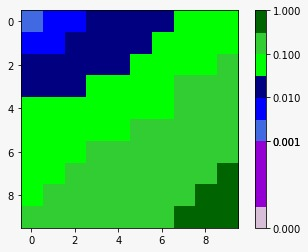
\includegraphics[width=0.5 \textwidth]{Images_Q2/Cluster.jpeg}
    \caption{Visualisation of the clusters.}
    \label{fig:figure5}
\end{figure}
In the end, we obtained a clustering with five different clusters. As seen in figure $\ref{fig:figure5}$, there are 5 different clusters with corresponding to a  different color. The representative color of each country is then used to color that country on the map. In the following figures, we can see how the world's total population has progressed decade wise from $1950$ to $2100$.
\begin{figure}[h!]
    \centering
    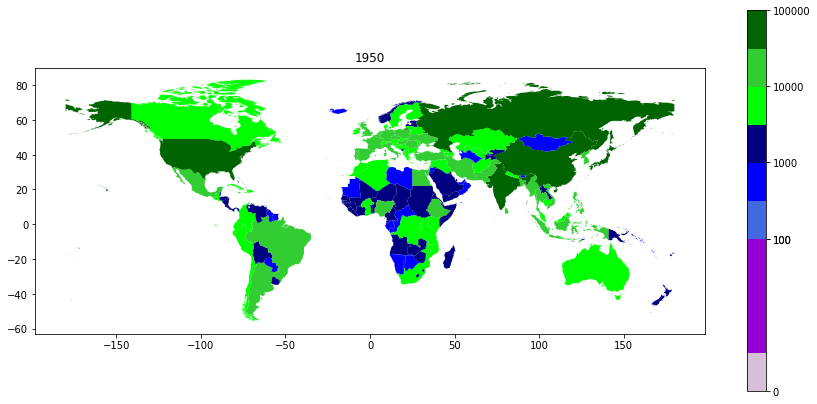
\includegraphics[width=0.9 \textwidth]{Images_Q2/1950.png}
    \caption{Worldwide Population in 1950}
    \label{fig:figure6}
\end{figure}
\newpage
\begin{figure}[h!]
    \centering
    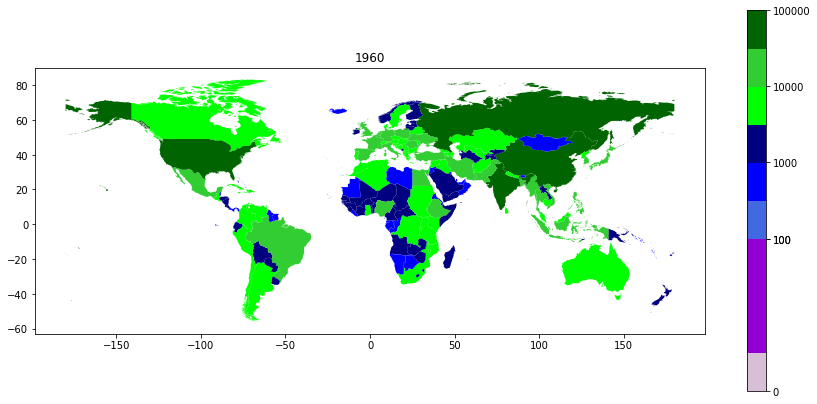
\includegraphics[width=0.9 \textwidth]{Images_Q2/1960.png}
    \caption{Worldwide Population in 1960}
    \label{fig:figure7}
\end{figure}
\begin{figure}[h!]
    \centering
    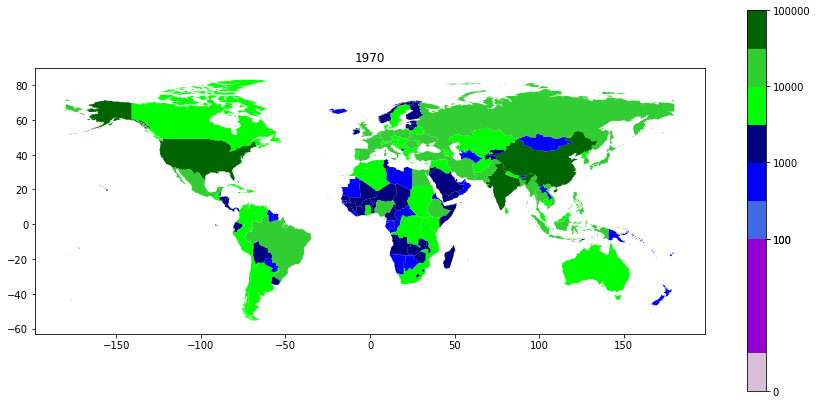
\includegraphics[width=0.9 \textwidth]{Images_Q2/1970.png}
    \caption{Worldwide Population in 1970}
    \label{fig:figure8}
\end{figure}
\newpage
\begin{figure}[h!]
    \centering
    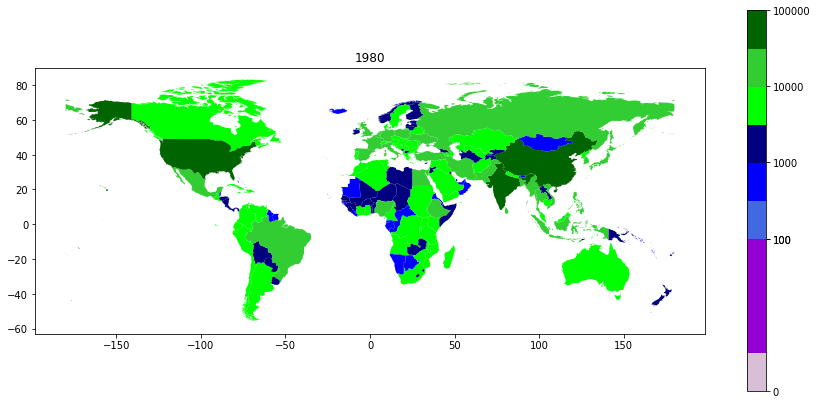
\includegraphics[width=0.9 \textwidth]{Images_Q2/1980.png}
    \caption{Worldwide Population in 1980}
    \label{fig:figure9}
\end{figure}
\begin{figure}[h!]
    \centering
    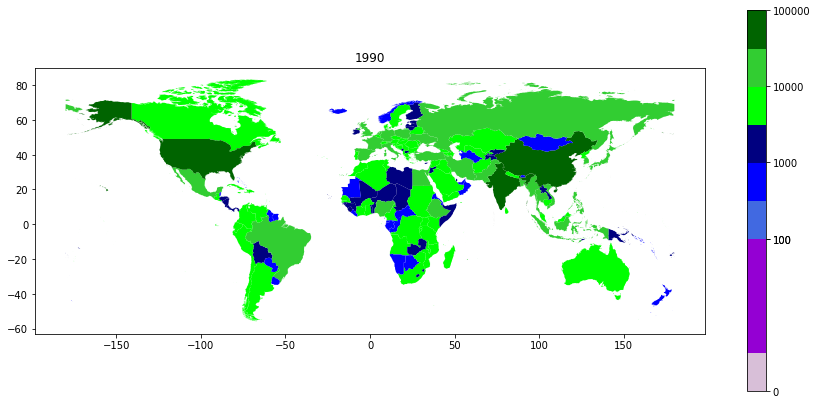
\includegraphics[width=0.9 \textwidth]{Images_Q2/1990.png}
    \caption{Worldwide Population in 1990}
    \label{fig:figure10}
\end{figure}
\newpage
\begin{figure}[h!]
    \centering
    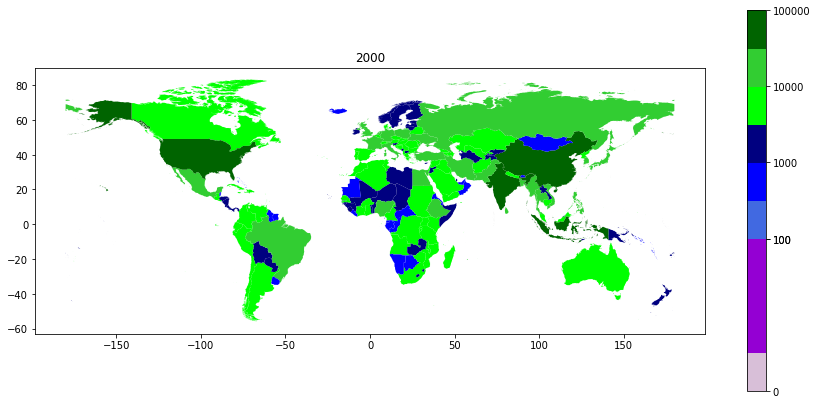
\includegraphics[width=0.9 \textwidth]{Images_Q2/2000.png}
    \caption{Worldwide Population in 2000}
    \label{fig:figure11}
\end{figure}
\begin{figure}[h!]
    \centering
    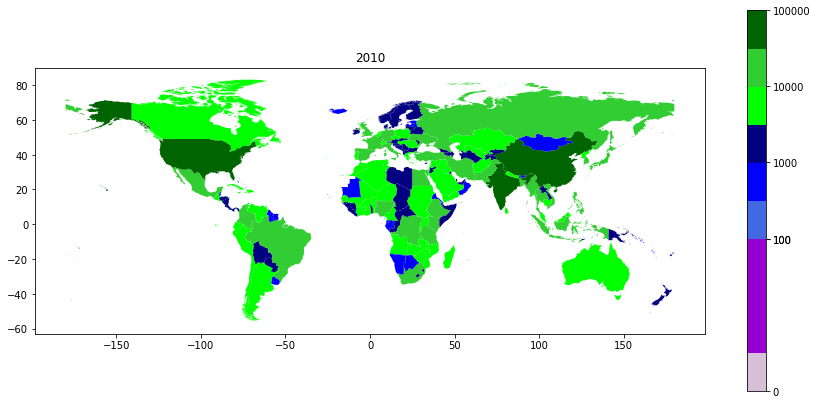
\includegraphics[width=0.9 \textwidth]{Images_Q2/2010.png}
    \caption{Worldwide Population in 2010}
    \label{fig:figure12}
\end{figure}
\newpage
\begin{figure}[h!]
    \centering
    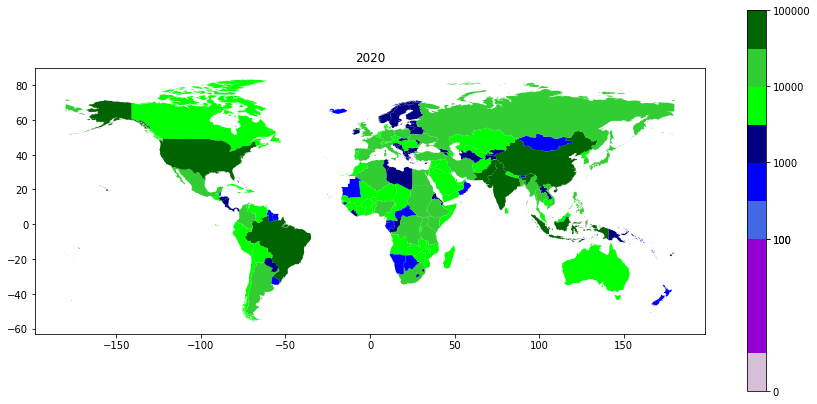
\includegraphics[width=0.9 \textwidth]{Images_Q2/2020.png}
    \caption{Worldwide Population in 2020}
    \label{fig:figure13}
\end{figure}
\begin{figure}[h!]
    \centering
    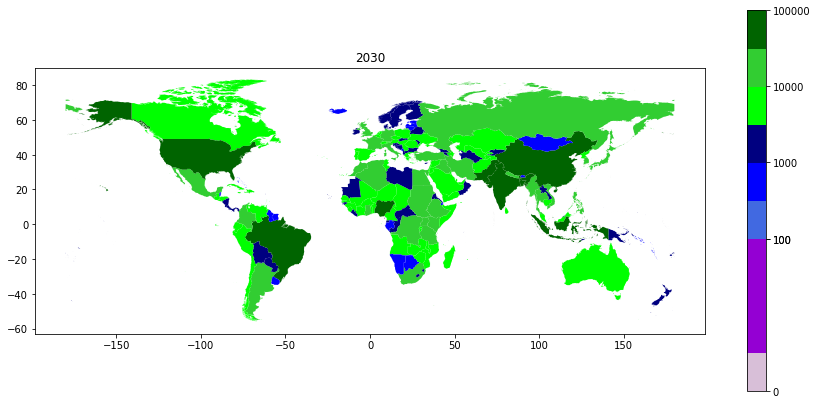
\includegraphics[width=0.9 \textwidth]{Images_Q2/2030.png}
    \caption{Worldwide Population in 2030}
    \label{fig:figure14}
\end{figure}
\newpage
\begin{figure}[h!]
    \centering
    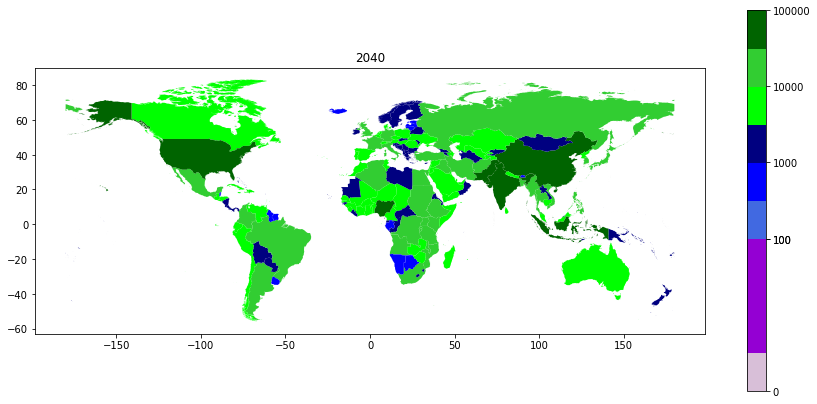
\includegraphics[width=0.9 \textwidth]{Images_Q2/2040.png}
    \caption{Worldwide Population in 2040}
    \label{fig:figure15}
\end{figure}
\begin{figure}[h!]
    \centering
    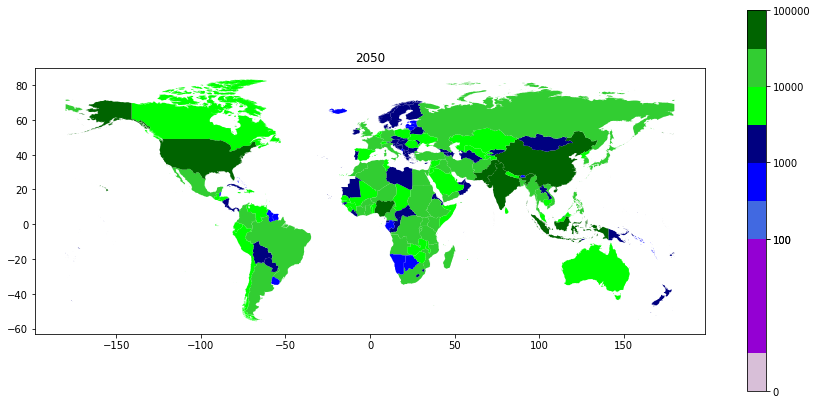
\includegraphics[width=0.9 \textwidth]{Images_Q2/2050.png}
    \caption{Worldwide Population in 2050}
    \label{fig:figure16}
\end{figure}
\newpage
\begin{figure}[h!]
    \centering
    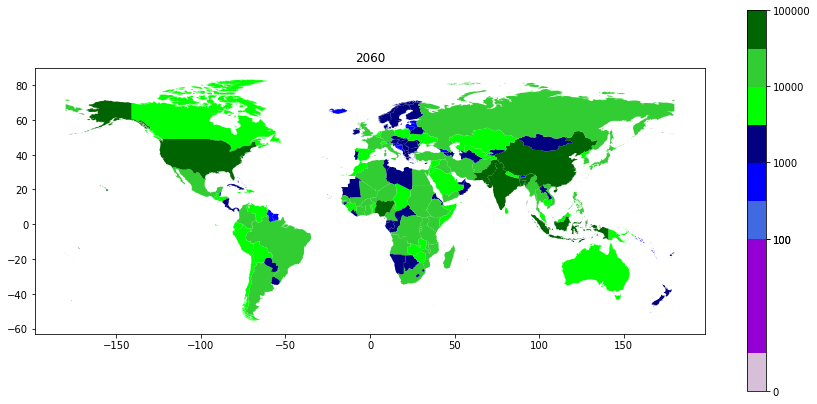
\includegraphics[width=0.9 \textwidth]{Images_Q2/2060.png}
    \caption{Worldwide Population in 2060}
    \label{fig:figure17}
\end{figure}
\begin{figure}[h!]
    \centering
    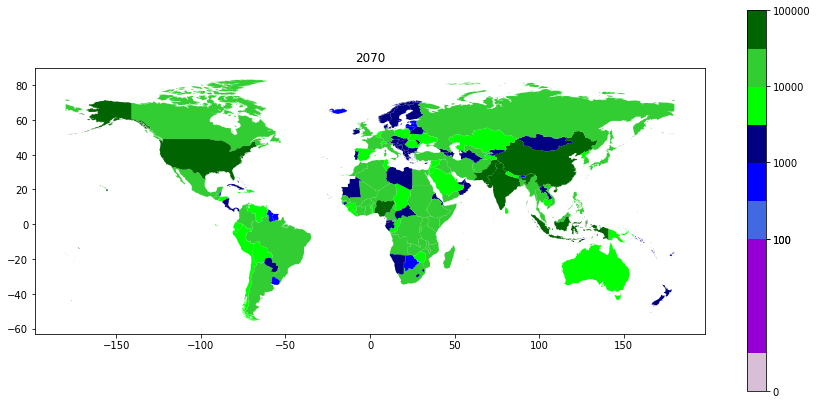
\includegraphics[width=0.9 \textwidth]{Images_Q2/2070.png}
    \caption{Worldwide Population in 2070}
    \label{fig:figure18}
\end{figure}
\newpage
\begin{figure}[h!]
    \centering
    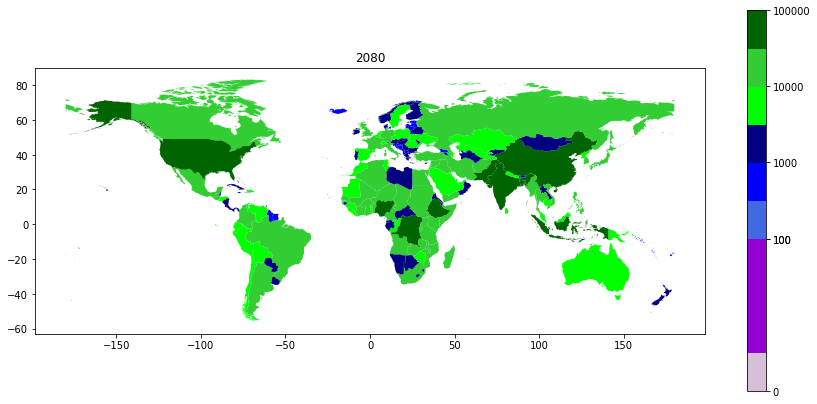
\includegraphics[width=0.9 \textwidth]{Images_Q2/2080.png}
    \caption{Worldwide Population in 2080}
    \label{fig:figure19}
\end{figure}
\begin{figure}[h!]
    \centering
    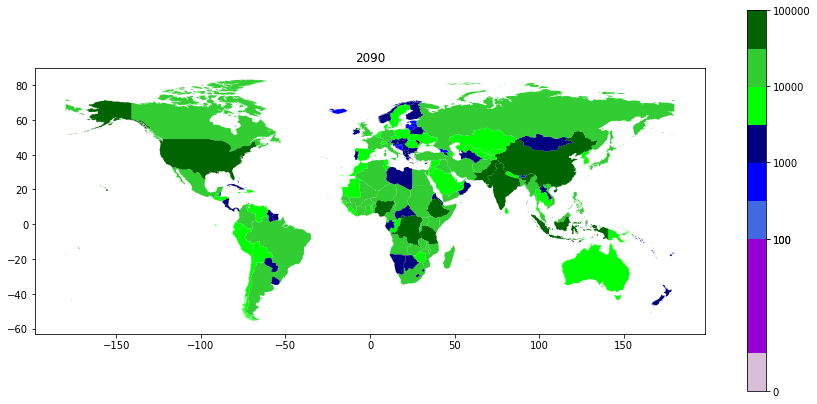
\includegraphics[width=0.9 \textwidth]{Images_Q2/2090.png}
    \caption{Worldwide Population in 2090}
    \label{fig:figure20}
\end{figure}
\newpage
\begin{figure}[h!]
    \centering
    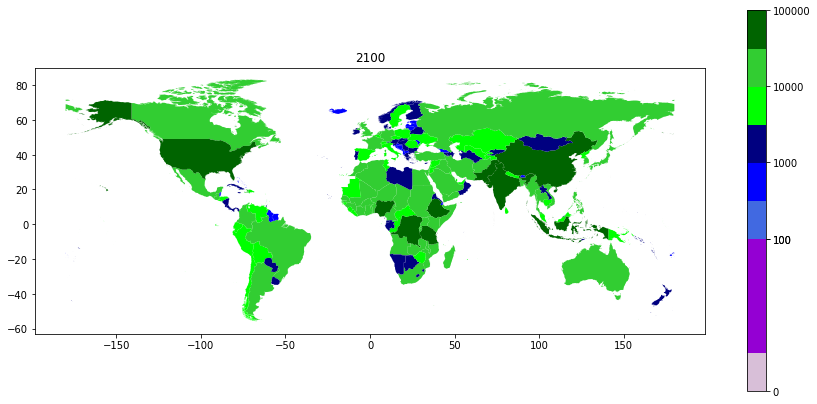
\includegraphics[width=0.9 \textwidth]{Images_Q2/2100.png}
    \caption{Worldwide Population in 2100}
    \label{fig:figure21}
\end{figure}

\begin{figure}[h!]
    \centering
    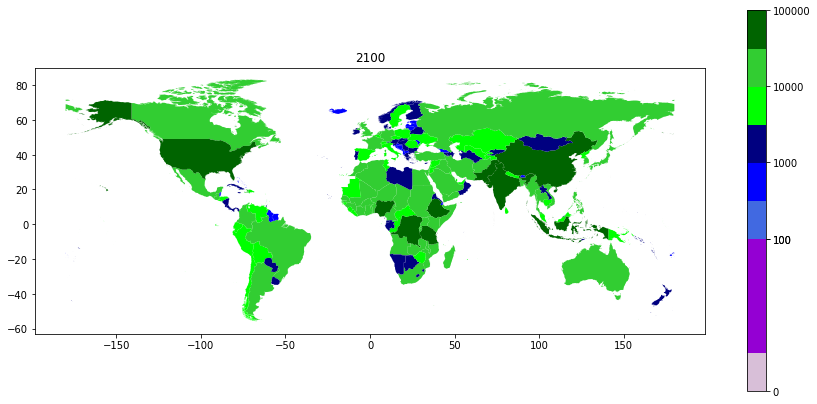
\includegraphics[width=0.9 \textwidth]{Images_Q2/2100.png}
    \caption{Worldwide Population in 2100}
    \label{fig:figure22}
\end{figure}

\section{Analysis}
In figure \ref{fig:figure6},we can see that there are blue patches which indicate a smaller world progression. However,as time progress these patches start into shades of green, which indicates a growing population. In addition to, we can see countries which have a dark green color such as China, USA, India, Pakistan . These are the countries which have the highest population in the world.
\end{document}

% timeeee